\documentclass[mathserif, xcolor=table]{beamer}
%\documentclass[mathserif,handout, xcolor=table]{beamer}
%\usetheme{Hannover}
%\usetheme{Pittsburgh}
\usetheme{boxes}
\setbeamercolor{structure}{fg=jblue!}


\usepackage{graphicx}  % Required for including images
\usepackage{array}
\usepackage{booktabs} % Top and bottom rules for tables
\usepackage{amsmath}
\usepackage{calc}
\usepackage{mathtools}
\usepackage{tabularx}
\usepackage{multirow}
\usepackage{pbox}
\usepackage{algorithm}
\usepackage{algorithmic}
\usepackage{caption}
%\usepackage{subcaption}


\def\1{\mathds{1}}
\def\D{\Delta}
\def\b{\beta}
\def\pd{\partial}
\def\grad{\nabla}
\def\Lo{\mathcal{L}}
\def\N{\mathbb{N}}
\def\At{{\tilde{A}}}
\def\Bt{{\tilde{B}}}
\def\Z{\mathcal{Z}}
\def\T{\mathcal{T}}
\def\C{\mathcal{C}}
\def\Lt{\tilde{L}}
\def\R{\mathbb{R}}
\def\X{\mathcal{X}}
\def\Y{\mathcal{Y}}
\def\I{\mathcal{I}}
\def\F{\mathcal{F}}
\def\w{\textbf{w}}
\def\x{\textbf{x}}
\def\wt{\tilde{\textbf{w}}}
\def\xt{\textbf{x}}
\def\v{\textbf{v}}
\def\u{\textbf{u}}
\def\k{\textbf{k}}
\def\d{\boldsymbol{\delta}}
\def\y{\textbf{y}}
\def\l{\ell}
\def\a{\alpha}
\def\vertspace{0.6em}
\def\train{\texttt{train}\hspace{1mm}}
\def\val{\texttt{val}\hspace{1mm}}
\def\test{\texttt{test}\hspace{1mm}}
\def\mthd{LatEm\hspace{1mm}}
\def\argmax{\mathop{\rm arg\,max}\limits}%    a math operator.
\def\argmin{\mathop{\rm arg\,min}\limits}%    a math operator.



\setbeamertemplate{footline}[text line]{%
  %\parbox{0.8\linewidth}{
   % \vspace*{-8pt}\insertshorttitle~(\insertshortauthor)
  %}
  \hfill%
  \parbox{0.15\linewidth}{
    \vspace*{-8pt}\raggedleft\insertframenumber
  }
}
\setbeamertemplate{navigation symbols}{}
%\setbeamertemplate{footline}[frame number]
\setbeamertemplate{navigation symbols}{}
\setbeamertemplate{frametitle}[default][left]
\setbeamercolor{itemize item}{fg=black}
\setbeamercolor{itemize subitem}{fg=black}

 \setbeamertemplate{itemize items}[circle]
\setbeamerfont{footline}{size=\footnotesize}
\setbeamerfont{section in toc}{size=\small}
\setbeamerfont{subsection in toc}{size=\footnotesize}


\definecolor{lgreen} {RGB}{180,210,100}
\definecolor{dblue}  {RGB}{20,66,129}
\definecolor{ddblue} {RGB}{11,36,69}
\definecolor{lred}   {RGB}{220,0,0}
\definecolor{nred}   {RGB}{224,0,0}
\definecolor{norange}{RGB}{230,120,20}
\definecolor{nyellow}{RGB}{255,221,0}
\definecolor{ngreen} {RGB}{98,158,31}
\definecolor{dgreen} {RGB}{78,138,21}
\definecolor{nblue}  {RGB}{28,130,185}
\definecolor{jblue}  {RGB}{20,50,100}

%\graphicspath{{../latEm_tpami/figures/}}
\def\X{\mathcal{X}}
\def\Y{\mathcal{Y}}

%%%%%%%%%%%%%%%%

\newlength{\depthofsumsign}
\setlength{\depthofsumsign}{\depthof{$\sum$}}
\newlength{\totalheightofsumsign}
\newlength{\heightanddepthofargument}

\newcommand{\nsum}[1][1.4]{% only for \displaystyle
    \mathop{%
        \raisebox
            {-#1\depthofsumsign+1\depthofsumsign}
            {\scalebox
                {#1}
                {$\displaystyle\sum$}%
            }
    }
}
%%%%%%%%%%%%%%%%%%%%%



%----------------------------------------------------------------------------------------
%	TITLE SECTION 
%----------------------------------------------------------------------------------------

\title{Practical session on Embeddings Applied to Zero-shot Learning} 
\author{Yongqin Xian \vspace{2mm}\\}
\institute{Max-Planck Institute for Informatics}
\date{12 September 2016}
%----------------------------------------------------------------------------------------



\begin{document}


%----------------------------------------------------------------------------------------
%	TITLE FRAME
%----------------------------------------------------------------------------------------

\begin{frame}
\color{jblue}\rule{4.3in}{0.02\paperwidth} \\ \vspace{-2mm}
\begin{minipage}{0.2\textwidth}

\includegraphics[width=0.6\textwidth,trim=0 -40 0 0]{minerva_solo.pdf}

\includegraphics[width=1.2\textwidth,trim=0 -300 0 0]{Logo_MPII}
\end{minipage}
\hfill
\begin{minipage}{0.5\textwidth} \hfill
%\includegraphics[width=0.5\textwidth,trim=0 30 -50 0]{iitk_vision} \vspace{2mm}

\includegraphics[width=0.4\textwidth,trim=0 -30 50 0]{SaarlandUni}
\end{minipage}
\titlepage
\end{frame}

%----------------------------------------------------------------------------------------
%	INTRO FRAME
%----------------------------------------------------------------------------------------
\begin{frame}{Outline}

\begin{itemize}
\item{Zero-shot Learning}
\item{Structural Joint Embedding}
\item{Demos}
\item{Latent Embedding}
\item{Demos}


\end{itemize}


\end{frame}

%----------------------------------------------------------------------------------------
%	Zero-shot Learning(ZSL) Problem FRAME
%----------------------------------------------------------------------------------------
\begin{frame}{Zero-shot Learning(ZSL) Problem}

Training phase: 
\begin{enumerate}
\item{Observed data set} 
\begin{equation*}
S = \{(x, y)| x \in X, y \in Y \}
\end{equation*}

\item{Extract image and class embeddings} 
\begin{equation*}
S_{\theta, \varphi} = \{(\theta(x), \varphi(y))| \theta(x) \in \X, \varphi(y) \in \Y \}
\end{equation*}
$\theta(x)$: image embedding, $\varphi(y)$: class embedding
\pause
\item{Using $S_{\theta, \varphi} $, learn function}
\begin{equation*}
f: X \rightarrow Y
\end{equation*}

\end{enumerate}
\pause

Testing phase: 
\begin{enumerate}
\item{Predict $x^*$ of unseen classes using $f(x^*)$} 

\end{enumerate}

\end{frame}

%----------------------------------------------------------------------------------------
%	INTRO FRAME
%----------------------------------------------------------------------------------------
%\begin{frame}{Structural Joint Embedding}
%SJE~[Akata et.al.'15]: \alert{single bilinear} compatibility
%\begin{itemize}
%	\item Not discriminative enough	
%\end{itemize}
%\begin{figure}
%\vspace{-4mm}
%\begin{center}
%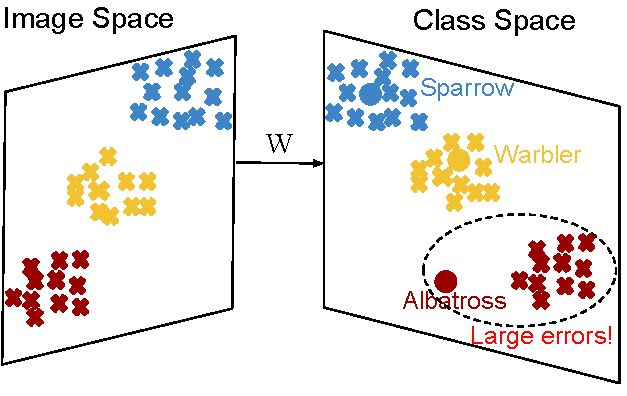
\includegraphics[width=0.7\textwidth]{linear_teaser}
%\end{center}
%\vspace{-6mm}
%\begin{equation*}
%F(x,y) = x^\top W y %
%\end{equation*}
%\vspace{-4mm}
%\\
%\textbf{Proposed solution}
%\begin{itemize}
%	\item Learn multiple linear mappings matrices
%	\item Non-linear~(piece-wise linear) model
%\end{itemize}

%\end{frame}

%----------------------------------------------------------------------------------------
%	SJE Frame
%----------------------------------------------------------------------------------------
\begin{frame}{Structural Joint Embedding}
\begin{center}
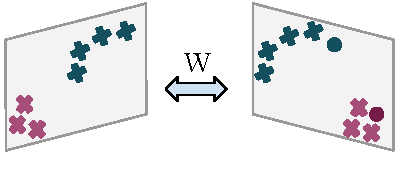
\includegraphics[width=0.7\textwidth]{SJE}
\end{center}
\vspace{-4mm}
\pause

Prediction function
\begin{equation*}
f(x; W) = \argmax_{y\in Y} \theta(x)^T W \varphi(y), 
\end{equation*}
\pause

Objective function
\begin{equation*}
    \min_W \frac{1}{N} \sum_{n=1}^{N} \max_{y\in Y \setminus \{y_n\}} \{0, \D(y_n,y) + \theta(x_n)^T W \varphi(y)-\theta(x_n)^T W \varphi(y_n)\},
\end{equation*}

\end{frame}

%----------------------------------------------------------------------------------------
%	SJE Frame
%----------------------------------------------------------------------------------------
\begin{frame}{Structural Joint Embedding}

\begin{algorithm}[H]
\begin{algorithmic}[1]
\STATE  Given $\T = \{(x, y)| x \in \R^{d_x}, y \in \R^{d_y}\}$ 
\STATE  Initialize $W$ randomly
\pause

\FOR{$t=1$ to $T$}
\FOR{$n=1$ to $|\T|$}
     		\STATE  Draw $(x_n$, $y_n) \in \T$
     		\pause

     		\STATE $y^* \leftarrow \argmax\limits_{y \in \Y \setminus \{y_n\}} x_n^\top W y$
     		     		\pause

      			\IF{$x_n^\top W y^* + 1 > x_n^\top W y_n $} 
					\STATE	$W \leftarrow W - \eta x_n (y^* - y_n)^\top$ 
        		\ENDIF
\ENDFOR
\ENDFOR
\end{algorithmic}
\caption*{Algorithm: SGD optimization of SJE }
\label{alg:seq}
\end{algorithm}


\end{frame}

%----------------------------------------------------------------------------------------
%	SJE Frame
%----------------------------------------------------------------------------------------
\begin{frame}{Demo}
Dataset: Animal with Attributes, train 40 cls, test 10 cls
\begin{itemize}
\item Task 1: Image Classification \\ 
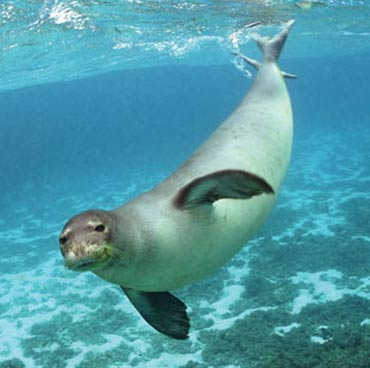
\includegraphics[width=0.1\textwidth]{seal}
\item Task 2: Image Retrieval
\end{itemize}
%\begin{enumerate}
%\item Image Classification 
%\item Image Retrieval
%\end{enumerate}

\begin{equation*}
	\argmax_{i} \theta(x_i)^\top W \varphi(y) 
\end{equation*}
%\center
%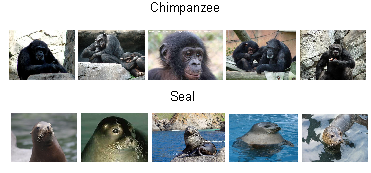
\includegraphics[width=0.7\textwidth]{sje_cont_AWA}

\end{frame}



%----------------------------------------------------------------------------------------
%	Latent Embeddings Method FRAME
%----------------------------------------------------------------------------------------
\begin{frame}{Latent Embeddings Method~(LatEm)}
\vspace{-4mm}
\begin{center}
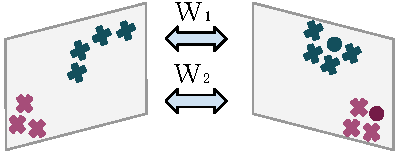
\includegraphics[width=0.7\textwidth]{Latem}
\end{center}
\vspace{-4mm}
\begin{equation*}
F(x,y) = \max_{1\leq i \leq K} \theta(x)^\top W_i \varphi(y)
\end{equation*}
\pause

%\end{equation*}
\begin{itemize}
	\item Learn a collection of matrices
	\item Selection of which one to use is latent
\end{itemize}

\end{frame}


%----------------------------------------------------------------------------------------
%	Latent Embeddings Method FRAME
%----------------------------------------------------------------------------------------
\begin{frame}{Latent Embeddings Method~(LatEm)}
Loss function
\begin{equation*}
    L(x_n,y_n) = \sum_{y \in \Y} \left[\D(y_n,y) + F(x_n,y) -F(x_n,y_n)\right]_+,
\end{equation*}
\pause

Objective function
\begin{equation*}
\frac{1}{N} \sum_{n=1}^{N} L(x_n, y_n).
\end{equation*}

\end{frame}

%----------------------------------------------------------------------------------------
%	Latent Embeddings Method Frame
%----------------------------------------------------------------------------------------
\begin{frame}{Latent Embeddings Method~(LatEm)}
\begin{algorithm}[H]
\small
\begin{algorithmic}[1]
\small
    \FORALL {$t=1$ to $T$} 
	\FORALL {$n=1$ to $|\T|$} 
      		\STATE  Draw $(x_n$,$y_n) \in \T$ and $y \in \Y \setminus \{y_n\}$ 
      		\pause

      			\IF {$F(x_n,y) + 1 > F(x_n,y_n)$} 
      			\pause

				\STATE $i^* \leftarrow \argmax\limits_{1\leq k\leq K} x_n^\top W_k y$
				\STATE $j^* \leftarrow \argmax\limits_{1\leq k\leq K} x_n^\top W_k y_n $  
				      			\pause

				\IF {$ i^* = j^*$} 
				\STATE $W_{i^*}^{t+1} \leftarrow W_{i^*}^{t} - \eta_t x_n (y - y_n)^\top$
				\ENDIF
				      			\pause

				\IF {$ i^* \neq j^*$} 
          			\STATE $W_{i^*}^{t+1} \leftarrow W_{i^*}^{t} - \eta_t x_n y^\top$ 
          			\STATE $W_{j^*}^{t+1} \leftarrow W_{j^*}^{t} + \eta_t x_n y_n^\top$ 
          			\ENDIF
        		\ENDIF
      \ENDFOR
    \ENDFOR
\end{algorithmic}
\caption*{Algorithm: SGD optimization of LatEm }
\label{alg:seq}
\end{algorithm}


\end{frame}


%----------------------------------------------------------------------------------------
%	Demo Frame
%----------------------------------------------------------------------------------------
\begin{frame}{Demo}


\end{frame}

%----------------------------------------------------------------------------------------
%	End Frame
%----------------------------------------------------------------------------------------
\begin{frame}{}
\center
\huge
Thank you!

\end{frame}



\end{document}


